\chapter{电子学：反馈、振荡器与信号采集}\label{ch:b2:feedback-oscillators}

把话筒靠得太近，对着它所驱动的扬声器，
大厅里便会充满啸叫：放大器听到了自己的声音，
一点微弱的噪声会迅速长成音调固定的尖啸。驯服之后，
同一个回路便是每一台时钟、收音机与合成器的核心——一个仅凭增益与滤波器便能产生正弦波的\emph{振荡器}。
第一册（本科一年级分册）用运算放大器构造了放大器、
滤波器和比较器；本章在它们外面闭合回路，
讨论回路何时稳定、何时振荡，构造两个振荡器——一个正弦式，
一个方波式——然后转向测得信号进入计算机的两种操作：
一是对它进行
\emph{采样}，二是借助
\emph{\omterm{prop:b2:feedback-oscillators:lockin}{同步检波}}将其从噪声中提取出来。

\begin{omfigure}
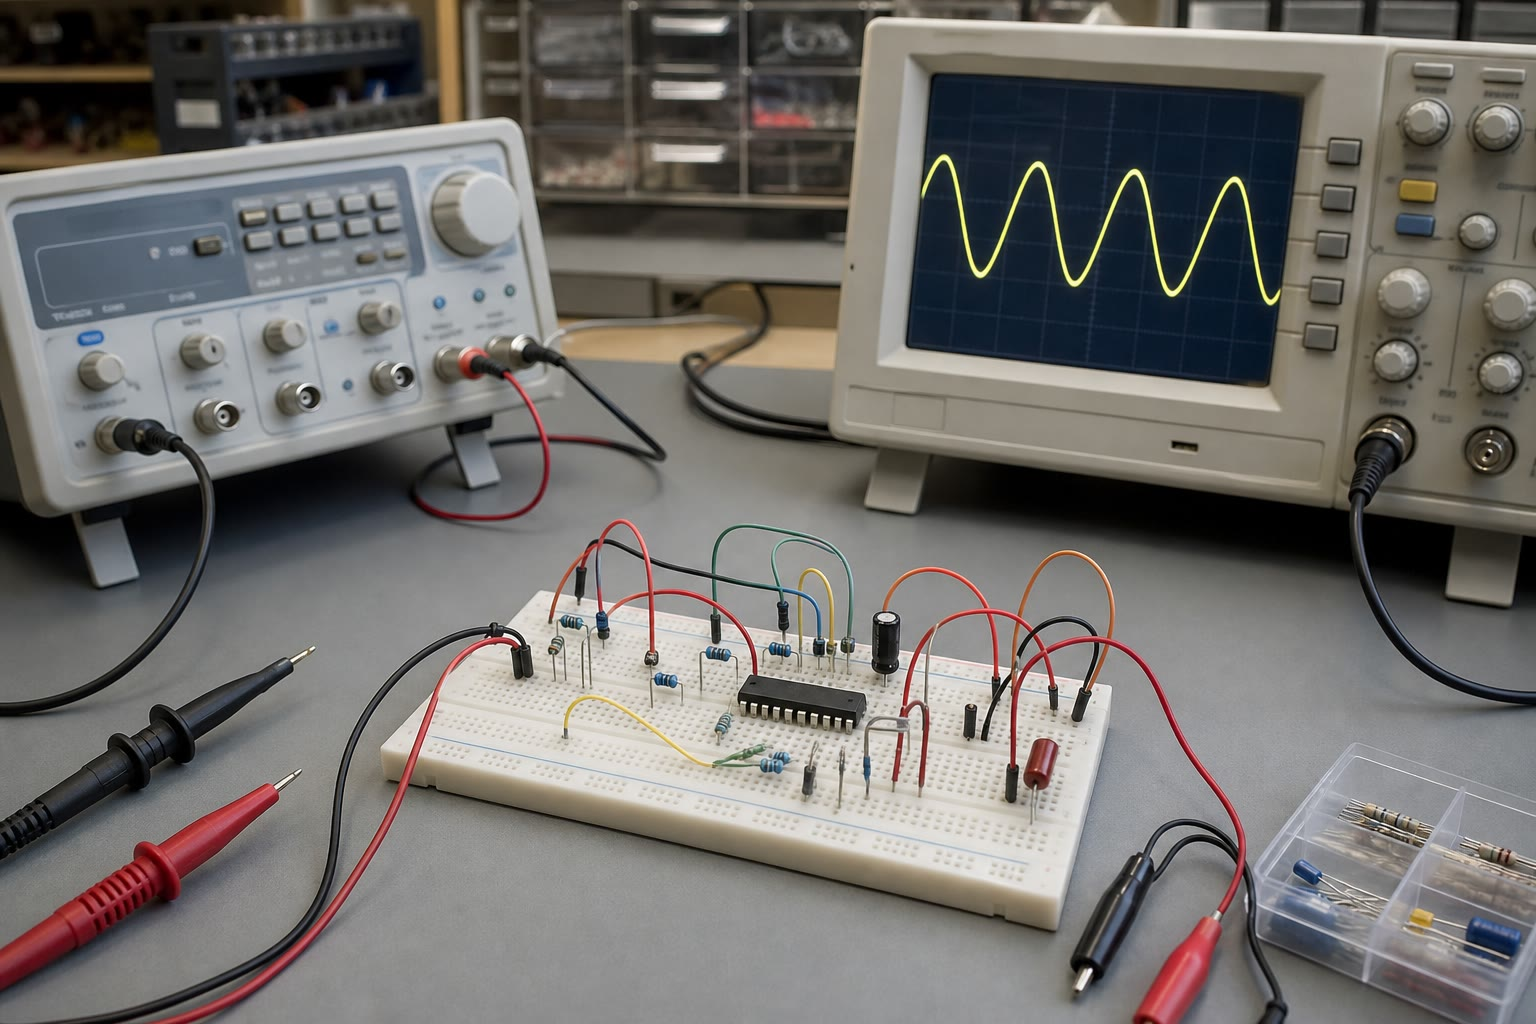
\includegraphics[width=0.58\linewidth]{images/book4/ai/b4-09-electronics-bench-oscillator.jpg}

{\small 面包板、函数发生器与示波器：这是闭合\omterm{def:b2:feedback-oscillators:loop}{反馈}回路的工作台，也是在放大器开始啸叫时发现它已变成振荡器的地方。}
\end{omfigure}


\section{反馈与稳定性}

\begin{definition}[闭环；环路增益]\label{def:b2:feedback-oscillators:loop}
\index{反馈}\index{环路增益}\index{闭环传递函数}
传递函数为 $\underline A(\jmath\omega)$ 的放大器接收输入 $\underline e$
与 $\underline\beta(\jmath\omega)\,\underline s$ 之和，
此处 $\underline s$ 为其自身输出（正反馈；若为负反馈，则将 $\beta$ 变号）。
称\emph{闭环}传递函数与
\emph{环路增益}分别为
\[
\underline H = \frac{\underline s}{\underline e} = \frac{\underline A}{1 - \underline A\,\underline\beta} ,
\qquad \underline T = \underline A\,\underline\beta .
\]
\end{definition}

\begin{theorem}[线性回路的稳定性；振荡条件]\label{thm:b2:feedback-oscillators:stability}
\index{稳定性（线性系统）}\index{巴克豪森条件}\index{特征方程}
将 $\jmath\omega$ 换成复变量 $p$，则回路的自由演化
由其\emph{\omterm{thm:b2:feedback-oscillators:stability}{特征方程}}的根决定
$1 - \underline A(p)\underline\beta(p) = 0$ 的根（$\underline H$ 的极点）：每个根
$p_i$ 对应一个模式 $\eu^{p_it}$。当所有
根的实部均为负（每个模式都衰减至零）时，回路\emph{稳定}；
当某个根的实部为正时，回路\emph{振荡}，振幅增长。
其分界为一对纯虚根 $\pm\jmath
\omega_0$，即持续的正弦振荡，满足
\[
\underline A(\jmath\omega_0)\,\underline\beta(\jmath\omega_0) = 1
\]
（称\emph{\omterm{thm:b2:feedback-oscillators:stability}{巴克豪森条件}}：在 $\omega_0$ 处，\omterm{def:b2:feedback-oscillators:loop}{环路增益}的模为一，相位为零）。
对于二阶分母 $ap^2 + bp + c$，
回路稳定，当且仅当 $a$、$b$、$c$ 同号。
\end{theorem}

\begin{proof}
回路的微分方程由 $\underline s(1 -
\underline A\underline\beta) = \underline A\underline e$ 出发，将 $\jmath\omega$ 的每一次幂
读作时间导数；其齐次解为 $\eu^{p_it}$，
其中 $p_i$ 为多项式的根。增长或衰减由
$\operatorname{Re}p_i$ 的符号决定；对二阶多项式，
当且仅当系数同号时其根的实部为负，
（根之和为 $-b/a$，根之积为 $c/a$）。
\omterm{thm:b2:feedback-oscillators:stability}{巴克豪森条件}即为存在根 $p = \jmath\omega_0$。
\end{proof}

\begin{remark}[振荡器的起振与停振]\label{rem:b2:feedback-oscillators:start}
振荡器的设计，使其在 $\omega_0$ 处的\omterm{def:b2:feedback-oscillators:loop}{环路增益}略\emph{大于}一：
开机时噪声中含有该频率成分，它按指数规律增长，而其他频率则逐渐消亡。
线性理论于是预言振幅无限增大；而实际上，
某种\emph{非线性}——放大器的饱和，
或刻意设置的非线性元件——
会随振幅增大而降低有效增益，直至
\omterm{def:b2:feedback-oscillators:loop}{环路增益}的平均值恰好为一：振幅于是稳定下来。每个实际振荡器，
就频率而言是线性回路，就振幅而言则是非线性回路；
限幅越平缓，
正弦波便越纯净。
\end{remark}

\section{维恩电桥振荡器}

\begin{proposition}[维恩电桥振荡器]\label{prop:b2:feedback-oscillators:wien}
\index{维恩电桥振荡器}\index{维恩网络}
同相接法的运算放大器，增益为 $K = 1 + R_2/R_1$，
将其输出经\emph{\omterm{prop:b2:feedback-oscillators:wien}{维恩网络}}\omterm{def:b2:feedback-oscillators:loop}{反馈}至 $+$ 输入端：
$R$ 与 $C$ 先串联，再与 $R$、$C$ 并联接地。
该网络的传递函数为
\[
\underline\beta(\jmath\omega) = \frac1{3 + \jmath(RC\omega - 1/RC\omega)} ,
\]
其为实数，最大值（$= 1/3$）在 $\omega_0 = 1/RC$ 处取得。\omterm{def:b2:feedback-oscillators:loop}{环路增益} $K\underline\beta$
在 $\omega_0$ 处，当 $K = 3$ 时等于一，此时电路维持一个正弦振荡，
其频率为
\[
f_0 = \frac1{2\pi RC} .
\]
电压 $v$ 位于 $+$ 输入端，满足
\[
\frac{\dd^2v}{\dd t^2} + \frac{3 - K}{RC}\,\frac{\dd v}{\dd t} + \frac{v}{R^2C^2} = 0 :
\]
当 $K < 3$ 时振荡衰减，当 $K > 3$ 时振荡增长（负阻尼），
时间常数为 $2RC/(K - 3)$，直至
运放饱和将其限幅。
\end{proposition}

\begin{proof}
分压关系：串联支路 $Z_s = R + 1/\jmath C\omega$，并联
支路 $Z_p = R/(1 + \jmath RC\omega)$；$\underline\beta = Z_p/(Z_s + Z_p)$，
化简后即得所给形式。环路方程为 $\underline v = \underline\beta K\underline v$，即
$[3 + \jmath(RC\omega - 1/RC\omega)]\underline v = K\underline v$；两边乘以 $\jmath\omega RC$，
并以 $\jmath\omega \to \dd/\dd t$ 替换，得 $R^2C^2\ddot v + (3 - K)RC\dot v + v = 0$。
其阻尼系数在 $K = 3$ 处变号。
\end{proof}

\begin{omfigure}
\begin{tikzpicture}[font=\small, x=1cm, y=1cm, >=Stealth, scale=0.9, every node/.style={transform shape}]
  \begin{scope}
    \node[draw, thick, minimum width=1.4cm, minimum height=0.8cm] (A) at (0,0) {$\underline A$};
    \node[draw, thick, minimum width=1.4cm, minimum height=0.8cm] (B) at (0,-1.7) {$\underline\beta$};
    \draw[thick] (-2.3,0) circle (0.2); \node at (-2.3,0) {$+$};
    \draw[thick, ->] (-3.2,0) -- (-2.5,0) node[above, pos=0.3, font=\footnotesize] {$\underline e$};
    \draw[thick, ->] (-2.1,0) -- (A.west);
    \draw[thick, ->] (A.east) -- (2.0,0) node[above, pos=0.6, font=\footnotesize] {$\underline s$};
    \draw[thick] (1.4,0) -- (1.4,-1.7) -- (B.east);
    \draw[thick, ->] (B.west) -- (-2.3,-1.7) -- (-2.3,-0.2);
    \node[font=\footnotesize] at (-0.3,-2.7) {$\underline H = \dfrac{\underline A}{1 - \underline A\underline\beta}$};
  \end{scope}
\end{tikzpicture}
\hfill
\begin{tikzpicture}[font=\small, scale=0.78, every node/.style={transform shape}]
    \draw (0,0) node[op amp, noinv input down] (oa) {};
    % negative feedback: R2 from output to - input, R1 from - input to ground
    \coordinate (M) at ($(oa.-)+(-0.7,0)$);
    \draw (oa.-) -- (M);
    \draw (M) to[R, l_=$R_1$] ++(-1.6,0) node[ground, rotate=-90]{};
    \draw (M) -- ++(0,1.4) coordinate (T) to[R, l=$R_2$] (T -| oa.out) -- (oa.out);
    % Wien network: from output down, series C and R to node P, P to + input; P to ground via R and via C
    \coordinate (P) at (-3.4,-2.3);
    \draw (oa.out) -- ++(0.6,0) coordinate (O) -- (O |- P) to[C, l=$C$] ++(-1.6,0) to[R, l=$R$] (P);
    \draw (P) -- (P |- oa.+) -- (oa.+);
    \draw (P) to[R, l_=$R$] ++(0,-1.6) node[ground]{};
    \draw (P) -- ++(-1.1,0) coordinate (Q) to[C, l_=$C$] ++(0,-1.6) node[ground]{};
    \draw (O) to[short, -o] ++(0.5,0) node[right, font=\footnotesize] {$s$};
\end{tikzpicture}

{\small 左：\omterm{def:b2:feedback-oscillators:loop}{反馈}环路——输出经
$\underline\beta$ 回送到放大器输入端。右：维恩桥
振子——同相放大器，增益为 $1 + R_2/R_1$，其
输出回送到其 $+$ 输入端，经串并联 $RC$
网络；当增益达到 3 时，以 $1/2\pi RC$ 的频率振荡。}
\end{omfigure}

\begin{example}[1 kHz 信号源]\label{ex:b2:feedback-oscillators:wiennumbers}
$R = \qty{15.9}{k\ohm}$，$C = \qty{10}{nF}$：$f_0 = \qty{1.00}{kHz}$。取 $R_1 =
\qty{10}{k\ohm}$，$R_2 = \qty{21}{k\ohm}$，$K = 3.1$：振幅
每增大 $\eu$ 倍所需时间为 $2RC/0.1 = \qty{3.2}{ms}$，由开关接通时的噪声起振，
几十毫秒内达到饱和；限幅后的正弦波
富含谐波。换用一只小型白炽灯泡代替 $R_1$，其
电阻随温度升高而增大，使 $K$ 恰好降至 $3$，
即在适中振幅处得到失真度小于 $0.1\%$ 的正弦波，
这正是最早的实验室信号发生器所用的电路。
\end{example}

\section{带迟滞的比较器；无稳态多谐振荡器}

\begin{proposition}[迟滞比较器]\label{prop:b2:feedback-oscillators:schmitt}
\index{迟滞比较器}\index{施密特触发器}
具有\emph{正}\omterm{def:b2:feedback-oscillators:loop}{反馈}的运算放大器——输出端接至 $+$ 输入端，
其间经分压器 $R_1$、$R_2$ 相连（此时 $+$ 输入端电位为 $\beta s$，其中
$\beta = R_1/(R_1 + R_2)$，信号 $e$ 加在 $-$ 输入端）
——它没有稳定的线性区：输出停留在 $+V_{\text{饱和}}$ 或
$-V_{\text{饱和}}$ 之一，并在以下条件下翻转：
\begin{align*}
&\text{由 } +V_{\text{饱和}} \text{ 变为 } -V_{\text{饱和}} \text{，条件是 } e \text{ 升至高于 } +\beta V_{\text{饱和}} ,\\
&\text{由 } -V_{\text{饱和}} \text{ 变为 } +V_{\text{饱和}} \text{，条件是 } e \text{ 降至低于 } -\beta V_{\text{饱和}} .
\end{align*}
两个阈值不同：\emph{迟滞}量 $2\beta V_{\text{饱和}}$ 使比较器
对小于该值的噪声不敏感，其在 $(e, s)$ 平面中的循环是一个
沿顺时针方向运行的矩形。
\end{proposition}

\begin{proof}
当 $s = +V_{\text{饱和}}$ 时，$+$ 输入端电位为 $+\beta V_{\text{饱和}}$；只要 $e < \beta V_{\text{饱和}}$，
输出就保持为正，$e$ 越过该值时即翻转——
此后 $+$ 输入端电位为 $-\beta V_{\text{饱和}}$，因此 $e$ 必须
降到该值以下才能使其翻回。（在线性区内，正\omterm{def:b2:feedback-oscillators:loop}{反馈}会使任何偏差增大，
即该状态是不稳定的。）
\end{proof}

\begin{proposition}[无稳态多谐振荡器]\label{prop:b2:feedback-oscillators:astable}
\index{无稳态多谐振荡器}\index{弛豫振子}
将\omterm{prop:b2:feedback-oscillators:schmitt}{迟滞比较器}的输出回送到其自身的 $-$ 输入端，
经一个 $RC$ 电路（$R$ 从 $s$ 接到 $-$ 输入端，$C$ 从该处
接到地）。电容器向 $\pm V_{\text{饱和}}$ 充电，
每当电压达到阈值便使比较器翻转：$s$ 处为方波，
$C$ 上为近似三角波，其周期为
\[
T = 2RC\,\ln\frac{1 + \beta}{1 - \beta} .
\]
当 $\beta = 1/2$ 时，$T = 2RC\ln3 \approx 2.2RC$。这类\emph{\omterm{prop:b2:feedback-oscillators:astable}{弛豫
振子}}可为微控制器提供时钟、使指示灯闪烁，
并产生函数发生器中的三角波和方波。
\end{proposition}

\begin{proof}
当 $s = +V_{\text{饱和}}$ 时，电容电压 $v_C$ 从
$-\beta V_{\text{饱和}}$ 向 $+V_{\text{饱和}}$ 按 $v_C = V_{\text{饱和}} - (1 + \beta)
V_{\text{饱和}}\eu^{-t/RC}$ 变化，电压达到 $+\beta V_{\text{饱和}}$ 时所经时间为 $RC\ln[(1 + \beta)
/(1 - \beta)]$；比较器翻转，随后是对称的半循环。
\end{proof}

\begin{omfigure}
\begin{tikzpicture}
\begin{axis}[omaxis, axis x line=middle, axis y line=middle, width=5.6cm, height=4.6cm,
    xlabel={$e$}, ylabel={$s$}, xmin=-1.6, xmax=1.6, ymin=-1.5, ymax=1.5,
    xtick=\empty, ytick=\empty, clip=false]
  \node[font=\scriptsize, anchor=north] at (axis cs:-0.5,-1.55) {$-\beta V_{\text{饱和}}$};
  \node[font=\scriptsize, anchor=north] at (axis cs:0.5,-1.55) {$\beta V_{\text{饱和}}$};
  \node[font=\scriptsize, anchor=east] at (axis cs:-1.55,1) {$V_{\text{饱和}}$};
  \node[font=\scriptsize, anchor=east] at (axis cs:-1.55,-1) {$-V_{\text{饱和}}$};
  \draw[dotted] (axis cs:-0.5,0) -- (axis cs:-0.5,-1.5); \draw[dotted] (axis cs:0.5,0) -- (axis cs:0.5,-1.5);
  \addplot[omDef, very thick] coordinates {(-1.5,1) (0.5,1)};
  \addplot[omDef, very thick, ->] coordinates {(0.5,1) (0.5,-1)};
  \addplot[omDef, very thick] coordinates {(0.5,-1) (-0.5,-1)};
  \addplot[omDef, very thick, ->] coordinates {(-0.5,-1) (-0.5,1)};
  \addplot[omDef, very thick] coordinates {(-0.5,-1) (1.5,-1)};
\end{axis}
\end{tikzpicture}
\hfill
\begin{tikzpicture}
\begin{axis}[omaxis, axis x line=middle, axis y line=left, width=8.0cm, height=4.6cm,
    xlabel={$t$}, ylabel={}, xmin=0, xmax=4.4, ymin=-1.4, ymax=1.4, xtick=\empty, ytick={-1,-0.5,0.5,1},
    yticklabels={$-V_{\text{饱和}}$, $-\beta V_{\text{饱和}}$, $\beta V_{\text{饱和}}$, $V_{\text{饱和}}$}, tick label style={font=\scriptsize}, samples=60,
    xlabel style={at={(axis description cs:1.0,0.5)}, anchor=west},
    legend style={font=\scriptsize, at={(0.5,1.02)}, anchor=south, legend columns=2, draw=none, fill=none}]
  \addplot[omThm, thick] coordinates {(0,1) (1.1,1) (1.1,-1) (2.2,-1) (2.2,1) (3.3,1) (3.3,-1) (4.4,-1)};
  \addplot[omDef, thick, domain=0:1.1] {1-1.5*exp(-x)};
  \addplot[omDef, thick, domain=1.1:2.2] {-1+1.5*exp(-(x-1.1))};
  \addplot[omDef, thick, domain=2.2:3.3] {1-1.5*exp(-(x-2.2))};
  \addplot[omDef, thick, domain=3.3:4.4] {-1+1.5*exp(-(x-3.3))};
  \legend{$s$（方波）, $v_C$}
\end{axis}
\end{tikzpicture}

{\small 左：滞回比较器的循环——两个阈值，
一个矩形按顺时针方向运行。右：\omterm{prop:b2:feedback-oscillators:astable}{无稳态多谐振荡器}——
电容器电压在两个阈值之间往返，输出为
方波。}
\end{omfigure}

\section{信号的采样}

\begin{theorem}[采样；奈奎斯特–香农准则]\label{thm:b2:feedback-oscillators:shannon}
\index{采样}\index{奈奎斯特–香农准则}\index{混叠}\index{抗混叠滤波器}
信号被\emph{采样}，是指只保留其在各时刻的取值 $s(nT_s)$，
这些时刻为 $nT_s$，$f_s = 1/T_s$ 称为\emph{采样率}。
采样后信号的频谱，是 $s$ 的频谱
在 $f_s$ 的每个整数倍附近重复出现。若信号的频谱被限制在
$f_{\max}$ 以下的信号可由其样本精确重建，当且仅当
下式成立：
\[
f_s > 2f_{\max} ;
\]
否则各副本相互重叠，频率 $f > f_s/2$ 的分量会
以\emph{混叠}频率 $|f - nf_s|$ 重新出现（其中整数 $n$
使其低于 $f_s/2$），与真正的低频分量无法区分。
因此，在任何采样器之前都要设置\emph{\omterm{thm:b2:feedback-oscillators:shannon}{抗混叠滤波器}}，
即一个滤除所有高于 $f_s/2$ 成分的低通滤波器。
\end{theorem}

\begin{proof}
采样即将 $s(t)$ 乘以一列窄脉冲，
该脉冲列的周期为 $T_s$，其傅里叶级数包含全部谐波 $nf_s$
（见本年度的数学分册）；将 $s$ 乘以 $\cos(2\pi nf_st)$
则使其频谱平移 $\pm nf_s$——由此得到各个副本。它们
当且仅当 $f_{\max} < f_s - f_{\max}$ 时互不重叠；截止频率为 $f_s/2$ 的低通滤波器
随后可精确恢复原频谱（在本阶段不加证明地承认）。关于混叠：
$\cos(2\pi ft)$ 与 $\cos(2\pi(f - nf_s)t)$ 在 $t = mT_s$
处的样本相同，因为 $2\pi nf_smT_s = 2\pi nm$。
\end{proof}

\begin{example}[车轮、光盘与示波器]\label{ex:b2:feedback-oscillators:alias}
以每秒 $24$ 幅画面拍摄的电影，以 \qty{24}{Hz} 的速率对世界采样：一个
有 $12$ 根辐条的车轮以每秒 $2.1$ 转的速度转动时，呈现某根辐条
$25.2$ 次，其中 $1.2$ 次超出 $f_s$——它似乎缓慢地向前转动，
而以每秒 $1.9$ 转的速度转动时则向后转动。光盘以
\qty{44.1}{kHz} 的速率采样，以重现高达 \qty{20}{kHz} 的声音，并设置陡峭的
\omterm{thm:b2:feedback-oscillators:shannon}{抗混叠滤波器}，位于 $20$ 至 \qty{22}{kHz} 之间。数字示波器
设置为 \qty{1}{MS/s} 时，会将 \qty{999}{kHz} 的正弦波显示为 \qty{1}{kHz} 的正弦波——
这是数字测量中的第一个陷阱。
\end{example}

\begin{omfigure}
\begin{tikzpicture}
\begin{axis}[omaxis, axis x line=middle, axis y line=none, width=13.6cm, height=4.0cm,
    xmin=0, xmax=10, ymin=-1.4, ymax=1.5, xtick=\empty, samples=400, xlabel={$t$},
    xlabel style={at={(axis description cs:1.0,0.5)}, anchor=west},
    legend style={font=\scriptsize, at={(0.5,1.02)}, anchor=south, legend columns=3, draw=none, fill=none}]
  \addplot[omDef, thick, domain=0:10] {cos(deg(2*pi*0.9*x))};
  \addplot[omThm, thick, dashed, domain=0:10] {cos(deg(2*pi*0.1*x))};
  \addplot[only marks, mark=*, mark size=1.6pt, black, samples=11, domain=0:10] {cos(deg(2*pi*0.9*x))};
  \legend{$f = 0.9f_s$, 混叠于 $0.1f_s$, 样本}
\end{axis}
\end{tikzpicture}

{\small 混叠：频率为 $0.9f_s$ 的正弦波与频率为 $0.1f_s$ 的正弦波经过
相同的样本点；一旦完成采样，二者便无法区分——因此需要
准则 $f_s > 2f_{\max}$。}
\end{omfigure}

\begin{remark}[量化]\label{rem:b2:feedback-oscillators:quantization}
\index{量化}\index{模数转换器}
\omterm{rem:b2:feedback-oscillators:quantization}{模数转换器}还会将每个样本舍入到
$2^N$ 个电平之一（$N$ 位）：舍入误差至多为半个台阶，相当于
方均根值为 $\Delta/\sqrt{12}$ 的噪声（台阶为 $\Delta$），且
动态范围（能超过该噪声的最大正弦波）约为 $6N + 2$ dB——
光盘的 $16$ 位对应 \qty{98}{dB}，$12$ 位
示波器对应 \qty{74}{dB}。采样率与分辨率是每台数字化仪标签上的
两个数字。
\end{remark}

\section{同步检波}

\begin{proposition}[同步（锁相）检波]\label{prop:b2:feedback-oscillators:lockin}
\index{同步检波}\index{锁相放大器}\index{解调}
频率已知的信号 $s(t) = A\cos(\omega_0t + \varphi)$ 淹没在
振幅大得多、分布于宽频带内的噪声 $n(t)$ 之中，
与频率相同的参考信号 $r(t) = \cos\omega_0t$ 相乘，
再通过截止频率为 $f_c \ll f_0$ 的低通滤波器：
\[
s(t)r(t) = \tfrac12A\cos\varphi + \tfrac12A\cos(2\omega_0t + \varphi)
\ \xrightarrow{\ \text{低通}\ }\ \tfrac12A\cos\varphi .
\]
输出为直流电压，它与信号的振幅成正比（并与信号相对于参考信号的相位的余弦成正比），
而噪声则被压缩至其频谱中
处于 $\pm f_c$ 范围内（以 $f_0$ 为中心）的部分
——带宽为 $2f_c$，它可以任意窄（时间常数为数秒的滤波器，
带宽可低至几分之一赫兹）。其他频率的分量
（频率为 $f$）被平移至 $f \pm f_0$，并被滤波器滤除。
\end{proposition}

\begin{proof}
$\cos a\cos b = \tfrac12[\cos(a - b) + \cos(a + b)]$；滤波器保留
信号的差频项，$2\omega_0$ 项以及每个
噪声分量（其频率 $f$ 平移至 $|f - f_0|$ 和 $f + f_0$），只有
原本在 $f_c$ 范围内（以 $f_0$ 为中心）的噪声才会落入低于 $f_c$ 的区域。
\end{proof}

\begin{omfigure}
\begin{tikzpicture}[font=\small, x=1cm, y=1cm, >=Stealth]
  \node[draw, thick, minimum width=1.5cm, minimum height=0.8cm] (S) at (0,0) {传感器};
  \node[draw, thick, circle, minimum size=0.7cm] (M) at (2.6,0) {$\times$};
  \node[draw, thick, minimum width=1.6cm, minimum height=0.8cm] (F) at (5.0,0) {低通};
  \node[draw, thick, minimum width=1.7cm, minimum height=0.8cm] (R) at (2.6,-1.9) {参考 $\omega_0$};
  \draw[thick, ->] (S) -- (M) node[above, pos=0.5, font=\footnotesize] {$s + n$};
  \draw[thick, ->] (M) -- (F);
  \draw[thick, ->] (F) -- (7.0,0) node[right, font=\footnotesize] {$\tfrac12A\cos\varphi$};
  \draw[thick, ->] (R) -- (M);
  \draw[thick, ->] (R.west) -- (-0.2,-1.9) -- (-0.2,-0.5) node[left, font=\footnotesize, pos=0.5] {调制};
\end{tikzpicture}
\hfill
\begin{tikzpicture}
\begin{axis}[omaxis, axis x line=bottom, axis y line=left, width=5.6cm, height=4.0cm,
    xlabel={$f$}, ylabel={}, xmin=0, xmax=3, ymin=0, ymax=1.3, xtick={1,2}, xticklabels={$f_0$, $2f_0$}, ytick=\empty, samples=200,
    xlabel style={at={(axis description cs:1.0,0.0)}, anchor=west}]
  \addplot[omExo!60, thick, domain=0:3] {0.35+0.1*sin(deg(11*x))+0.08*cos(deg(23*x))};
  \addplot[omThm, very thick] coordinates {(1,0) (1,1.1)};
  \addplot[omDef, thick, fill=omDef!30, domain=0.9:1.1] {1.2} \closedcycle;
  \node[font=\scriptsize, omDef, anchor=west] at (axis cs:1.15,1.15) {保留};
  \node[font=\scriptsize] at (axis cs:2.2,0.6) {噪声};
\end{axis}
\end{tikzpicture}

{\small 同步检测：传感器的输出，即信号加宽带
噪声，与信号自身频率的参考信号相乘，
再经低通滤波；只有 $f_0$ 附近窄带内的噪声
（阴影部分）得以保留，信号则以直流电平输出。}
\end{omfigure}

\begin{example}[寻找微伏信号]\label{ex:b2:feedback-oscillators:microvolt}
光电二极管在其光被斩波时输出 \qty{10}{\micro V} 的信号，
斩波频率为 \qty{1}{kHz}，其上叠加有 \qty{50}{nV/\sqrt{Hz}} 的白噪声，
带宽为 \qty{100}{kHz}（有效值为 \qty{16}{\micro V}，比信号还大）。经
同步检测，滤波器的时间常数为 $\tau = \qty{1}{s}$（噪声
带宽为 $1/4\tau = \qty{0.25}{Hz}$），噪声为 $50\,\text{nV} \times \sqrt{0.25}
= \qty{25}{nV}$：信噪比为 $400$——代价是
每个数据点需等待数秒。同一技巧在此称为
\emph{\omterm{prop:b2:feedback-oscillators:lockin}{解调}}，可从调幅无线电载波中恢复音乐，
也可从调制\omterm{prop:b2:feedback-oscillators:lockin}{解调}器中恢复数据。
\end{example}

\begin{method}[设计测量链]\label{met:b2:feedback-oscillators:method}
(1) 将待测量以远离噪声的频率 $f_0$ 进行调制
（斩波器、交流电桥）。(2) 以覆盖
$f_0$ 的带宽进行放大。(3) 取测量所能承受的最长时间常数的滤波器进行同步检测：
噪声按
$1/\sqrt\tau$ 下降。(4) 以高于慢输出带宽两倍的速率对其采样，
先经抗混叠滤波，位数足以满足
所需分辨率。(5) 用已知信号检验测量链，并检查其中
有无振荡：每个带\omterm{def:b2:feedback-oscillators:loop}{反馈}的放大器都是潜在的
振荡器。
\end{method}

\section{练习}

\begin{exercise}[$\star$]\label{exo:b2:feedback-oscillators:1}
\omterm{prop:b2:feedback-oscillators:wien}{维恩电桥振荡器}，$R = \qty{10}{k\ohm}$，$C = \qty{10}{nF}$：
求频率、所需增益；$R_1$、$R_2$ 的取值，使 $K = 3.05$，且 $R_1 =
\qty{10}{k\ohm}$；振幅增长的时间常数。哪些元件
决定频率，哪些决定起振？
\end{exercise}

\begin{exercise}[$\star$]\label{exo:b2:feedback-oscillators:2}
\omterm{prop:b2:feedback-oscillators:schmitt}{迟滞比较器}，$V_{\text{饱和}} = \qty{\pm 13}{V}$，$R_1 = \qty{1.0}{k\ohm}$，
$R_2 = \qty{4.0}{k\ohm}$：求阈值与迟滞宽度。一个
过零的带噪信号，噪声为 \qty{2}{V}：每次过零时输出
切换几次？分别考虑有迟滞与无迟滞两种情况。
\end{exercise}

\begin{exercise}[$\star$]\label{exo:b2:feedback-oscillators:3}
\omterm{prop:b2:feedback-oscillators:astable}{无稳态多谐振荡器}，$R = \qty{10}{k\ohm}$，$C = \qty{100}{nF}$，$\beta = 0.5$：
求周期与频率；频率为 \qty{1.0}{kHz} 时的 $R$；电容器上三角波的
振幅；$T$ 在 $\beta$ 提高到 $0.9$ 时如何变化？
\end{exercise}

\begin{exercise}[$\star$]\label{exo:b2:feedback-oscillators:4}
(a) CD 以 \qty{44.1}{kHz} 采样：求可再现的最高频率。(b) 一个
\qty{30}{kHz} 的超声波漏入录音中：它会以何频率
出现？(c) 一个有 $8$ 根辐条的车轮，以 \qty{25}{images/s} 拍摄，
它以 $3.2$ 转/秒转动：求表观运动。(d) 一台示波器以 \qty{10}{MS/s}
采样，显示出一个干净的 \qty{100}{kHz} 正弦波；真实信号可能是哪些
其他频率？
\end{exercise}

\begin{exercise}[$\star\star$]\label{exo:b2:feedback-oscillators:5}
具有下列特征多项式的环路：(a) $p^2 + 3p + 2$，(b) $p^2 - p +
4$，(c) $p^2 + 4$，(d) $p^3 + 2p^2 + 2p + 1$，(e) $p^3 + p + 1$：求根或
讨论其根；哪些环路稳定、哪些振荡、哪些增长？
（对三次式，由实部的符号推理：例如证明 (e)
有一个实负根与两个实部为正的复根，
利用根的和与积。）
\end{exercise}

\begin{exercise}[$\star\star$]\label{exo:b2:feedback-oscillators:6}
\emph{\omterm{prop:b2:feedback-oscillators:wien}{维恩网络}。}(a) 由分压器推导 $\underline\beta(\jmath\omega)$。
(b) 画出（草图）其模与相位；证明相位仅在
$\omega_0$ 处为零，且此时模为 $1/3$。(c) 写出增益为 $K$ 时环路的
微分方程，并讨论 $K < 3$、$K = 3$、$K > 3$ 的情形。
(d) 取 $K = 3.2$，从 \qty{1}{mV} 的噪声出发，需要多长时间
幅度才能达到 \qty{10}{V}？为何最终幅度与
初始噪声无关？
\end{exercise}

\begin{exercise}[$\star\star$]\label{exo:b2:feedback-oscillators:7}
\emph{三角波发生器。}一个积分器（运算放大器，$R$，$C$）的输入由
\omterm{prop:b2:feedback-oscillators:schmitt}{迟滞比较器}的方波输出 $\pm V_{\text{饱和}}$ 提供，该比较器的输入
是积分器的输出；比较器阈值为
$\pm V_{\text{饱和}}R_1/R_2$。(a) 证明积分器输出为三角波，
并求其斜率。(b) 周期 $T = 4RCR_1/R_2$。(c) 数值：$R = \qty{10}{k\ohm}$，
$C = \qty{10}{nF}$，$R_1/R_2 = 0.5$。(d) 说明它作为函数发生器时，相对于简单的
\omterm{prop:b2:feedback-oscillators:astable}{无稳态多谐振荡器}的优点。
\end{exercise}

\begin{exercise}[$\star\star$]\label{exo:b2:feedback-oscillators:8}
\omterm{rem:b2:feedback-oscillators:quantization}{量化}。(a) $16$ 位转换器在 $\pm\qty{1}{V}$ 范围内：求步长、
\omterm{rem:b2:feedback-oscillators:quantization}{量化}噪声有效值及以 dB 为单位的动态范围。(b) $12$ 位、
\qty{1}{MS/s}：求比特率；$8$ 位、\qty{1}{GS/s}（快速
示波器）的情形同样求解。(c) 将 \qty{1}{mV} 信号输入 $16$ 位转换器，共有多少
个\omterm{rem:b2:feedback-oscillators:quantization}{量化}台阶？转换器之前应做何处理？(d) 为何优质音频
系统在\omterm{rem:b2:feedback-oscillators:quantization}{量化}之前要加入抖动（即添加少量噪声）？
\end{exercise}

\begin{exercise}[$\star\star$]\label{exo:b2:feedback-oscillators:9}
一信号含有 \qty{1.0}{kHz} 与 \qty{9.0}{kHz} 两个分量，并以
\qty{10}{kS/s} 的速率采样。(a) 各分量分别出现在何处？(b) 若加入
一阶 $RC$ \omterm{thm:b2:feedback-oscillators:shannon}{抗混叠滤波器}，截止频率 $f_c = \qty{2}{kHz}$，
在 \qty{9}{kHz} 处以 dB 计的衰减量为多少；若需要 \qty{40}{dB}，是否足够？(c)
所需滤波器阶数（衰减 $\approx 20n$ dB 每十倍频程）；
或者，采用一阶滤波器时所需的采样率。(d)
为何现代转换器要进行过采样并以数字方式滤波？
\end{exercise}

\begin{exercise}[$\star\star\star$]\label{exo:b2:feedback-oscillators:10}
\emph{锁相放大。}输入 $A\cos(\omega_0t + \varphi) + n(t)$ 乘以 $\cos\omega_0t$
再经时间常数为 $\tau$ 的一阶低通滤波。(a) 直流
输出。(b) 证明频率为 $f = f_0 + \delta f$ 的噪声分量经滤波后
幅度减小为 $1/\sqrt{1 + (2\pi\delta f\tau)^2}$ 倍；
由此推出等效噪声带宽 $B = 1/4\tau$（可承认 $\int_0^\infty
\dd x/(1 + x^2) = \pi/2$）。(c) \qty{1}{\micro V} 的信号混在 \qty{1}{mV} 有效值的
白噪声中，带宽为 \qty{10}{kHz}：求噪声密度；$\tau$ 取何值时
信噪比为 $10$；并求测量时间。(d) 一个 \qty{50}{Hz} 的拾取干扰，幅度为 \qty{1}{mV}，
污染输入，取 $f_0 = \qty{1}{kHz}$：它流向何处，
衰减幅度为多少（$\tau = \qty{1}{s}$ 时）？
\end{exercise}

\begin{exercise}[$\star\star\star$]\label{exo:b2:feedback-oscillators:11}
\emph{石英。}石英晶体在其共振频率附近表现为一条
串联的 $L$、$C$、$r$ 支路（$L = \qty{8000}{H}$，$C = \qty{3.0}{fF}$，$r =
\qty{30}{k\ohm}$），与 $C_0 = \qty{1.5}{pF}$ 并联。(a) 求串联谐振
频率与品质因数 $Q = L\omega_0/r$。(b) 为何以其构成的振荡器能将频率稳定在
$10^6$ 分之一以内，而维恩电桥的
频率却漂移达百分之几（可考虑相位斜率 $\dd\varphi/\dd\omega$，
共振附近\omterm{def:b2:feedback-oscillators:loop}{反馈}网络的 $\sim 2Q/\omega_0$）？(c) 手表用的
石英晶体（频率为 \qty{32768}{Hz}）经 $2^{15}$ 分频后：求结果；
其频率的变化规律为 $-0.04\,\text{ppm}\,(T - \qty{25}{\degreeCelsius})^2$，求
在 \qty{5}{\degreeCelsius} 时每月的误差。(d) 为何选用 \qty{32768}{Hz} 而
不是 \qty{1}{MHz}？
\end{exercise}

\begin{exercise}[$\star\star\star$]\label{exo:b2:feedback-oscillators:12}
\emph{负电阻。}运算放大器中，$R_2$ 自输出端接至 $-$
输入端，$R_1$ 自 $-$ 输入端接地，$R$ 自输出端接至 $+$ 输入端；
研究 $+$ 输入端与地之间所见的二端网络（线性
区）。(a) 证明它等效为电阻 $-RR_1/R_2$。(b) 将此
二端网络跨接于一并联 $LC$ 电路两端，该电路含损耗电阻
$R_p$（并联），列出电压方程，并求持续振荡的
条件与频率。(c) 取数值：$L
= \qty{10}{mH}$，$C = \qty{100}{nF}$，$R_p = \qty{50}{k\ohm}$；选取 $R$，$R_1 =
R_2$。(d) 是什么限制了振幅，以及本振荡器
与维恩电桥相比如何？
\end{exercise}

\section{问题：锁相测量链}

\begin{problem}[{周末问题——从参考振荡器到
数字化结果：测量十微伏光信号，噪声为
毫伏量级的噪声}]
\label{pb:b2:feedback-oscillators:1}

用光电二极管测量一束微弱的光。该光经旋转轮
斩波，斩波频率为 $f_0 = \qty{1.00}{kHz}$，使光电二极管的
输出是幅值为 $A = \qty{10}{\micro V}$、频率为 $f_0$ 的正弦信号（经过
第一级放大器之后），其上叠加着谱密度
$e_n = \qty{50}{nV/\sqrt{Hz}}$ 的白噪声，带宽为 \qty{100}{kHz}，另有
幅值为 \qty{1.0}{mV}、频率为 \qty{50}{Hz} 的市电拾取干扰。斩波器本身的频率
由一\omterm{prop:b2:feedback-oscillators:wien}{维恩电桥振荡器}设定。

\medskip
\noindent\textbf{第一部分——参考振荡器。}
维恩电桥，$C = \qty{10}{nF}$，运算放大器在 $\pm\qty{12}{V}$ 处饱和。
\begin{enumerate}
  \item 求 $R$，使 $f_0 = \qty{1.00}{kHz}$。
  \item 推导\omterm{prop:b2:feedback-oscillators:wien}{维恩网络}的传递函数，并验证
        其在 $f_0$ 处相位为零、模为 $1/3$。
  \item 对增益 $K$ 写出回路的微分方程；
        当 $K = 3.15$ 时，求振幅增长为原来的 $1000$ 倍所需的时间。
  \item 振幅最终受饱和限制：描述
        波形，并说明其谐波对作为参考的信号为何重要。
  \item 以热敏电阻代替 $R_1$（其电阻随升温而减小
        ）或灯泡（电阻随之增大）：哪一种能将增益稳定在 3，
        并说明如何实现？
  \item 电容器随温度漂移 $+1\%$：求新的频率。
        为何此时斩波器仍能用于测量（参考振荡器
        须做到什么）？
  \item \omterm{prop:b2:feedback-oscillators:wien}{维恩网络}的品质因数约为 $1/3$，这
        对频率纯度意味着什么，与石英
        （$Q \sim 10^5$）相比？
\end{enumerate}

\medskip
\noindent\textbf{第二部分——信号与噪声。}
\begin{enumerate}[resume]
  \item 求在整个 \qty{100}{kHz} 带宽内白噪声的有效值；
        求放大器输出端的信噪比。
  \item 加入品质因数 $Q = 10$、中心位于 $f_0$ 的带通滤波器
        （噪声带宽 $\approx f_0/Q$），求噪声有效值与信噪比。
        为何仅此还不足以进行精确测量（考虑
        漂移以及 \qty{50}{Hz} 干扰）？
  \item 为何以 \qty{1}{kHz} 对光斩波，而不直接测量直流
        光电流？（放大器的 “$1/f$” 噪声在
        几百赫兹以下增大。）
  \item 若斩波轮产生方波而非正弦调制，则信号
        幅值如何：\omterm{prop:b2:feedback-oscillators:lockin}{锁相放大器}保留哪一次谐波、
        其幅值为多少（单位幅值方波基波的傅里叶系数为 $4/\pi$
        ）？
  \item 光电二极管还接收到 \qty{100}{Hz} 的室内光
        （荧光灯所致）：整个链路对它如何处理？
\end{enumerate}

\medskip
\noindent\textbf{第三部分——同步检测。}
放大后的信号与参考信号 $\cos(2\pi f_0t)$ 相乘，
再经时间常数为 $\tau$ 的一阶低通滤波器滤波。
\begin{enumerate}[resume]
  \item 求仅有信号时乘法器的输出（信号与参考之间的相位为 $\varphi$
        ），并求其中的直流项。
  \item 求滤波器对 $2f_0$ 项的衰减，取 $\tau = \qty{1}{s}$
        （以\omterm{def:b2:sound-waves:decibel}{分贝}计）。
  \item 等效噪声带宽为 $1/4\tau$；求输出端的噪声有效值
        （$\tau = \qty{1}{s}$ 时）及信噪比；$\tau = \qty{10}{s}$ 时亦同。
  \item \qty{50}{Hz} 的拾取干扰最终流向何处，
        其在 $\tau = \qty{1}{s}$ 时的衰减为多少？
  \item 相位 $\varphi$ 未知：若 $\varphi = \qty{60}{\degree}$，将损失什么？
        试描述双通道（同相与正交）\omterm{prop:b2:feedback-oscillators:lockin}{锁相放大器}，
        并说明它如何恢复 $A$，而与 $\varphi$ 的取值无关。
  \item 求测量的响应时间（达到终值的 $99\%$ 所需的时间
        ），取 $\tau = \qty{1}{s}$，并说明其所体现的权衡。
  \item 参考信号漂移至 \qty{1001}{Hz}，而斩波器仍保持在
        \qty{1000}{Hz}：求\omterm{prop:b2:feedback-oscillators:lockin}{锁相放大器}的输出；并说明为何参考信号必须
        取自斩波器本身。
\end{enumerate}

\medskip
\noindent\textbf{第四部分——数字化。}
\begin{enumerate}[resume]
  \item \omterm{prop:b2:feedback-oscillators:lockin}{锁相放大器}的输出由计算机采样，求
        $\tau = \qty{1}{s}$ 时的最低采样率（取输出带宽为 $1/2\pi\tau$）；给出一个
        合适的选择。
  \item 另一种做法是将原始 \qty{1}{kHz} 信号直接数字化，
        在软件中完成检测：求最低采样率。噪声
        延伸至 \qty{100}{kHz}——采样前须做什么，
        以及在 \qty{100}{kHz} 处的衰减为多少（采样率为
        \qty{20}{kS/s}，四阶滤波器截止频率为 \qty{5}{kHz}，
        滚降为 \qty{80}{dB} 每十倍频程）？
  \item 一个 $16$ 位转换器，量程为 $\pm\qty{1}{V}$：求步长；\qty{10}{\micro V}
        信号经 $1000$ 倍放大后占多少步长，噪声
        是有益还是有害？
  \item 数字锁相：计算机将每个采样值乘以
        $\cos(2\pi f_0nT_s)$，并对 $N$ 个采样值取平均。在 \qty{20}{kS/s}
        采样率下，求 \qty{1}{s} 平均所需的 $N$；白噪声被降低了多少倍，
        是否与模拟滤波器的相同？
  \item 以 \qty{999}{S/s} 的采样率对 \qty{1}{kHz} 信号采样，计算机
        看到的是什么？这与\omterm{prop:b2:feedback-oscillators:lockin}{锁相放大器}自身
        的原理有何联系？
  \item 用表格总结整条链路：各级分别对信号做了什么，
        对噪声又做了什么。
\end{enumerate}
\end{problem}
